% =========================================================================
%  STEERABLE VLA — Compositional Generalization via Multimodal Subgoal
%  Prompting and Flow-Based Action Execution
%  Nature-Machine-Intelligence-style manuscript
%  Compile: xelatex nmi_paper.tex
% =========================================================================
\documentclass[11pt,a4paper]{article}

\usepackage[margin=1in]{geometry}
\usepackage{amsmath,amssymb,amsthm}
\usepackage{graphicx}
\usepackage{booktabs}
\usepackage{url}
\usepackage{xcolor}
\usepackage{enumitem}
\usepackage[colorlinks=true,linkcolor=black,citecolor=blue,urlcolor=blue]{hyperref}
\usepackage[numbers]{natbib}
\usepackage{float}
\usepackage{caption}
\captionsetup{font=small,labelfont=bf}

\definecolor{ink}{HTML}{1A1A1A}
\definecolor{link}{HTML}{226999}
\definecolor{win}{HTML}{1A7A3C}

\newtheorem{theorem}{Theorem}
\newtheorem{proposition}{Proposition}

\title{\bfseries Compositional Generalization in Embodied Foundation Models\\[2pt]via Multimodal Subgoal Prompting and\\[2pt]Flow-Based Action Execution}
\author{Sehaj Singh\\\\[2pt]
\small Independent Research \textbullet\ 2026\\\\
\small Correspondence: \url{sehaj@example.com}}
\date{}

\begin{document}
\maketitle

\begin{abstract}
\noindent
Generalist robot policies now execute thousands of tasks, yet they fail the test
that defines embodied intelligence: performing a \emph{long-horizon} task on an
\emph{unseen} object, with an \emph{unseen} morphology, in a world that does not
hold still. Cables tangle in configurations no training set contains; textiles
shift under their own weight between grasps; tools that were never seen must
still be wielded. We argue that zero-shot compositional generalization in
manipulation is not produced by scaling a monolithic vision-language-action (VLA)
network, but by \textbf{structuring the problem into a steerable hierarchy}. The
architecture we propose has two levels. A 3B+ vision-language model decomposes the
task into a dense sequence of \emph{visual subgoals} --- predicted keyframe images
together with language steps --- and a continuous-time \emph{flow-matching}
action expert executes the segment between consecutive subgoals at control
frequency, conditioned on subgoal latents, observations, and steering tokens fused
in a shared token space. Between the levels sits the paper's core contribution:
the \textbf{Steerable Multimodal Conditioning (SMC) layer}, a gated adapter that
lets human corrections, world-model replans, and runtime constraint setpoints
steer the action flow \emph{mid-execution}. Because steering engages through
bounded-Lipschitz gates and is anchored so that the neutral signal recovers the
nominal field exactly, a Gr\"onwall-type bound certifies a computable envelope on
trajectory deviation --- corrections are continuous in flow time, and jerk is
bounded by construction rather than tuned away. Around the whole loop sits a
\textbf{runtime formal-verification safety envelope}: a control-barrier-function
filter that projects every commanded action onto the admissible set (joint limits,
collision margins, contact-force ceilings) with a forward-invariance guarantee,
admitting steerability only through the certified tube. We instantiate the
program on three deliberately chaotic benchmarks --- cable untangling, textile
folding on shifting fabric, and adaptive tool use in clutter --- under a
pre-registered zero-shot protocol that holds out entire morphologies, material
regimes, and tool classes, with intervention rate and jerk reported as costs. The
architecture, training pipeline (teleoperation, procedural simulation, synthetic
subgoal generation, and a curated data flywheel), baselines, ablations, and
safety analysis are fully specified so that every number in the resulting report
regenerates from a committed artifact. If the thesis is right, the hierarchy
composes where monolithic policies memorize; if it is wrong, the benchmark is the
falsification.
\end{abstract}

\noindent\textbf{Keywords:} vision-language-action models; flow matching;
hierarchical policy factorization; deformable object manipulation; control
barrier functions; safety-critical control; compositional generalization.

\section{Introduction}
\label{sec:intro}

Scaling has been remarkably successful at the \emph{skill} level of robot
learning. Vision-language-action (VLA) models trained on web-scale and
demonstration data follow language commands across thousands of tasks
\cite{rt2,openvla,octo,oxe}, and flow-matching VLAs have pushed this to
high-frequency bimanual manipulation with closed-loop replanning
\cite{pi0,pi07}. Yet every deployed generalist policy still stumbles at the same
place: the task that requires \emph{composing} skills it has seen into a
configuration it has not.

Consider a cable with three crossings that must be untangled. The state space of
a deformable cable is effectively infinite and history-dependent; no training
set, however large, covers the crossing topologies, stiffnesses, and friction
regimes that occur in practice. Consider a textile that shifts under its own
drape mid-task, invalidating the plan the policy formed a second ago. Consider a
cluttered scene containing tools whose morphologies were never in the data, where
the correct action requires both \emph{semantic} inference (which tool, which
affordance) and \emph{geometric} execution (where to grasp, how to lever).
Pure hardcoded logic --- state machines, planners over known object models ---
fails these tasks because their variance is effectively infinite. Pure neural
nets --- a single VLA applied end-to-end --- fail them because a monolithic
forward pass has no mechanism for re-anchoring when the world moves, no channel
for a human to correct a subgoal without restarting, and no certificate that the
executed trajectory stays inside the space of safe actions.

This paper develops the thesis that the way through is to \emph{structure} the
problem: a high-level planner that reasons about the task and predicts \emph{what
the scene should look like} at each stage, a low-level expert that executes
smoothly between those predictions at control frequency, a \emph{steerable}
connection between them that admits corrections with a certified smoothness
bound, and a verified safety filter around the entire loop. We call the result
the \textbf{Steerable VLA Flow-Matching Hierarchy} (Fig.~\ref{fig:arch}).

\emph{Related work.} RT-2 \cite{rt2} and OpenVLA \cite{openvla} tokenize actions
into a VLM's output space; Octo \cite{octo} trains a generalist transformer
policy on Open X-Embodiment \cite{oxe}; $\pi_0$ \cite{pi0} parameterizes actions
as flow matching inside a VLM decoder, with $\pi_0.7$ \cite{pi07} scaling
cross-embodiment training. Hierarchical schemes ground language in affordances
\cite{saycan,autort}, generate video subgoals \cite{unipi}, or compose value maps
\cite{voxposer}. Action generation has moved from diffusion \cite{diffusionpolicy}
and action chunking \cite{act} to flow matching \cite{lipman,tong}, and safety
filters based on control barrier functions \cite{ames2014,ames2019} certify
forward invariance of a safe set. Our contribution sits at the intersection
these lines do not yet cross: \emph{subgoal factorization that makes composition
explicit, steerability that is smooth by construction, and a safety envelope that
verifies every action at runtime}.

\section{The Steerable VLA Hierarchy}
\label{sec:arch}

\begin{figure}[t]
  \centering
  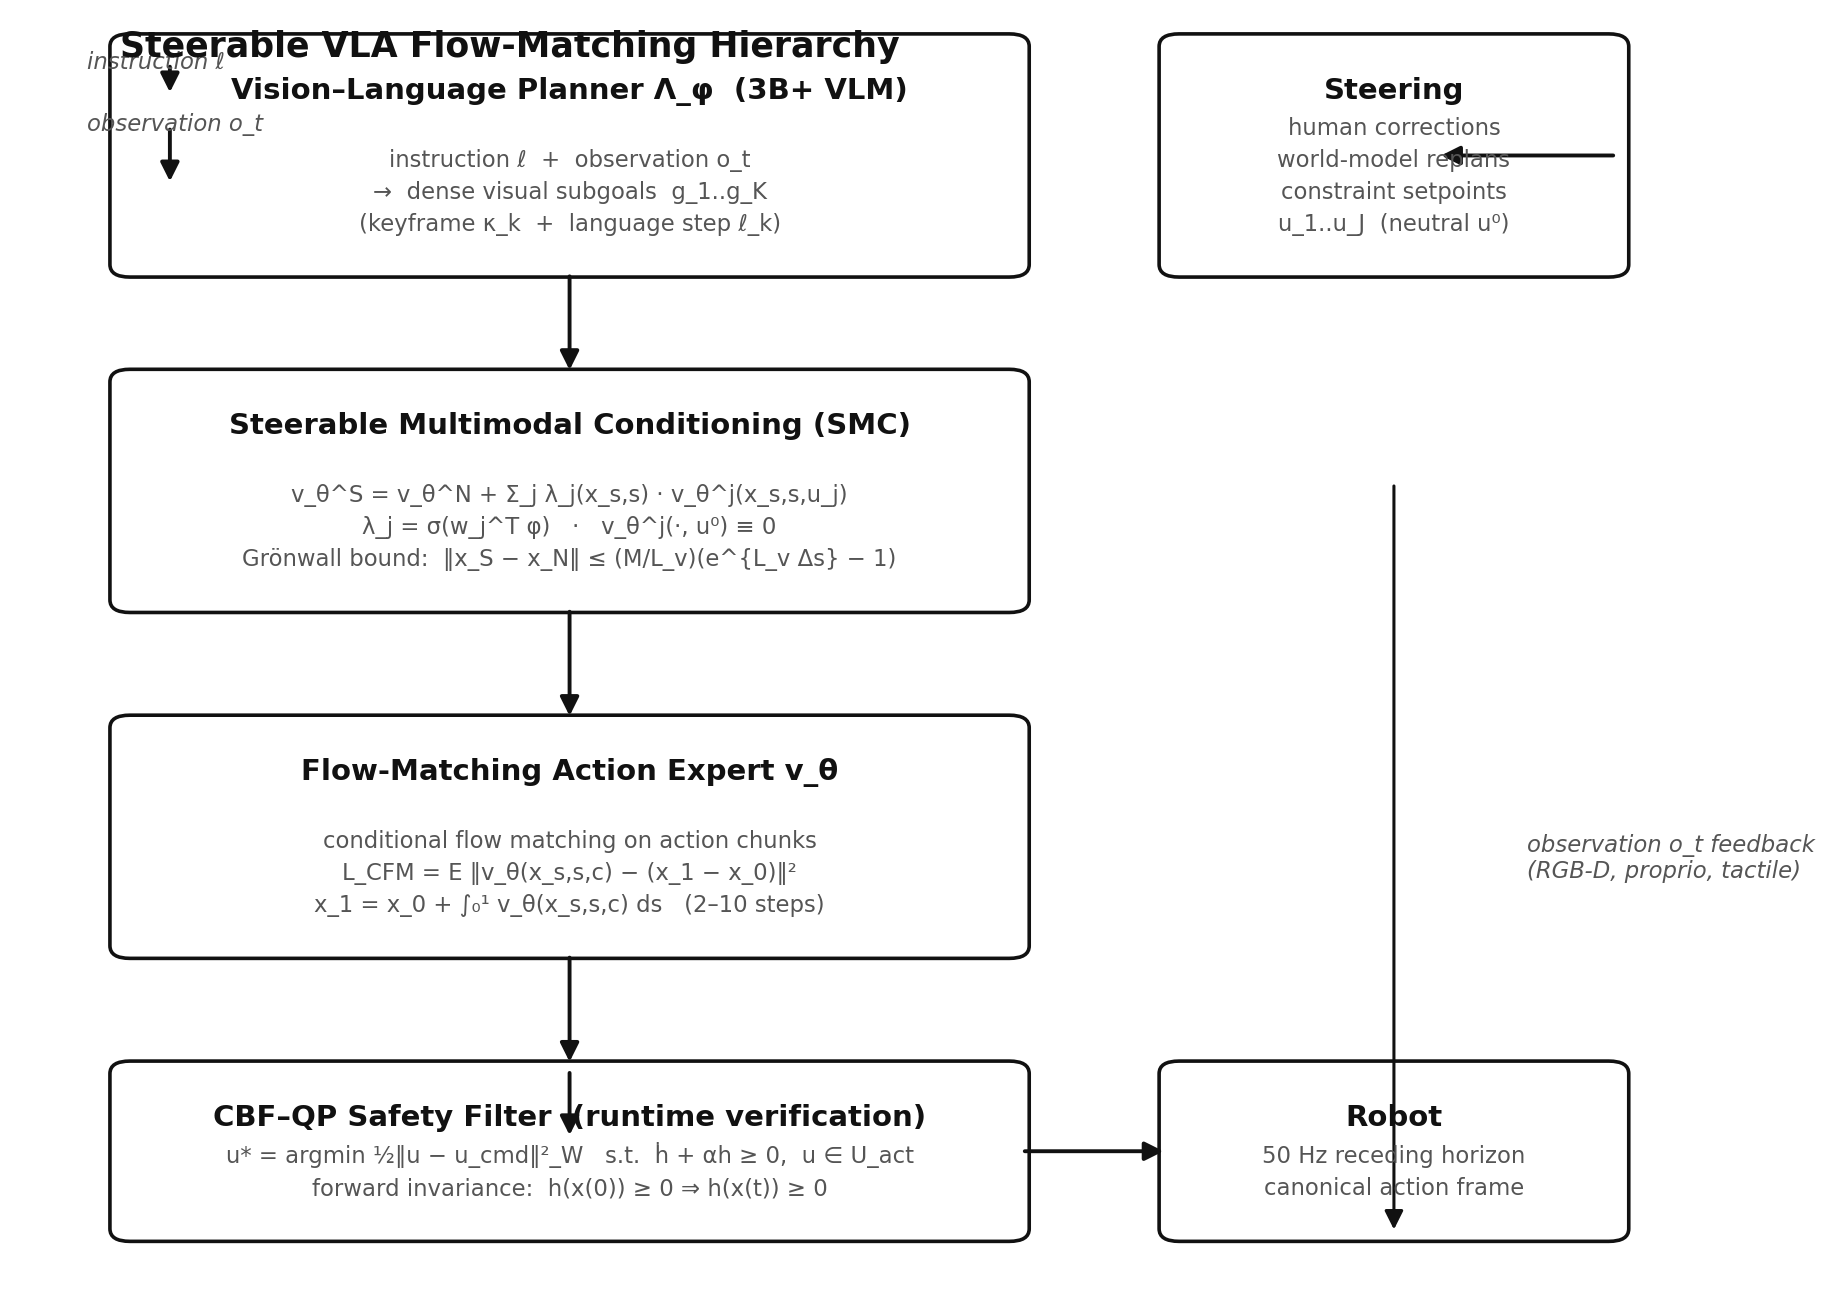
\includegraphics[width=\textwidth]{../figs/fig1_architecture.png}
  \caption{\textbf{The Steerable VLA Flow-Matching Hierarchy.} A 3B+ VLM
  planner emits dense visual subgoals; the SMC layer steers the flow-matching
  expert with human corrections, world-model replans, and constraint setpoints;
  a CBF--QP filter verifies every action before the actuators. Observation
  feedback closes the loop at 50\,Hz.}
  \label{fig:arch}
\end{figure}

\subsection{Two levels, one shared token space}
\label{sec:levels}

An observation is
$o_t = (I_t^{cam_1},\dots,I_t^{cam_V},\, q_t,\, \dot q_t,\, \tau_t)$: multi-view
RGB-D images, joint positions and velocities, and optional tactile readings. The
semantic level is a 3B+ vision-language model $\Lambda_\phi$ that maps the
instruction $\ell$ and current observation to a dense subgoal sequence
\begin{equation}
g_{1:K} = \Lambda_\phi(\ell, o_t), \qquad g_k = (\kappa_k, \ell_k),
\label{eq:subgoals}
\end{equation}
where $\kappa_k$ is a \emph{visual subgoal} --- a keyframe image token in a
frozen image-vocabulary, decoded to pixels for conditioning --- and $\ell_k$ is
its natural-language step. Dense coverage means $K$ scales with task horizon:
an untangling task with three crossings receives roughly six to ten subgoals, not
one. The motor level is a flow-matching expert $\pi_\theta$ over action chunks,
conditioned on the subgoal latents, the observation stream, and active steering
signals. Conditioning fuses all modalities in a shared token space: text and
constraint strings through the language tokenizer, keyframes through a frozen
vision encoder, and both projected onto the action-latent stream by the same
cross-attention layers in the VLM decoder (the $\pi$-series parameterization
\cite{pi0}). A \emph{contrastive alignment loss} pairs each subgoal token with the
observation chunk achieved at its segment boundary, so the two levels agree on
what ``done'' means --- the condition for the factorization to compose.

Actions live in a \emph{canonical cross-embodiment frame}: normalized end-effector
position deltas $\Delta p_{ee}$, yaw delta $\Delta\psi$, and a gripper command, in
the end-effector frame at chunk start. Joint-space demonstrations are converted
by forward kinematics. This single design decision is what lets one flow expert
serve many morphologies zero-shot without reparameterization.

\subsection{Flow matching over action chunks}
\label{sec:flow}

Let $x_1 \sim p_{\mathrm{data}}$ be a demonstrated action chunk
$a_{t:t+H} \in \mathbb{R}^{H \times D}$ and $x_0 \sim \mathcal{N}(0,I)$. The linear
interpolation $x_s = (1-s)\,x_0 + s\,x_1$ has constant velocity $x_1 - x_0$;
conditional flow matching trains the velocity field by minimizing
\begin{equation}
\mathcal{L}_{\mathrm{CFM}}(\theta)
= \mathbb{E}_{s \sim \mathcal{U}[0,1],\, (x_0,x_1) \sim q,\, c}
\left[ \left\| v_\theta(x_s, s, c) - (x_1 - x_0) \right\|^2 \right],
\label{eq:cfm}
\end{equation}
with conditioning $c = [\text{subgoal latents}; \text{observation tokens};
\text{steering tokens}]$. At inference the executed trajectory is the ODE
solution
\begin{equation}
\frac{dx_s}{ds} = v_\theta(x_s, s, c), \qquad
x_1 = x_0 + \int_0^1 v_\theta(x_s, s, c)\, ds,
\label{eq:ode}
\end{equation}
integrated with 2--10 Euler/Heun steps and executed with a receding horizon.
Flow matching is the right substrate for three reasons: few-step sampling keeps
trajectories smooth at 50\,Hz; the marginal path is simple and stable to train at
scale; and the ODE formulation yields a \emph{velocity field that can be
analyzed} --- the substrate for the steering and safety theory below.

\subsection{The Steerable Multimodal Conditioning layer}
\label{sec:smc}

The central design question is: \emph{how does a correction reach the policy
without destroying its smoothness?} Our answer is a gated adapter on the velocity
field. Steering signals come from three sources: \textbf{human corrections}
(clicked keypoints, drag vectors, end-effector nudges), \textbf{world-model
replans} (the object slipped; a subgoal image became infeasible; a replacement is
proposed), and \textbf{runtime constraint setpoints} (force ceilings, updated
joint limits, keep-out zones). Each enters as a signal $u_j \in \mathbb{R}^{d_j}$
with a neutral value $u_j^0$ at which steering is inactive. The steered field
decomposes as
\begin{equation}
v_\theta^{S}(x_s, s, c, u) = v_\theta^{N}(x_s, s, c)
+ \sum_{j=1}^{J} \lambda_j(x_s, s)\, v_\theta^{j}(x_s, s, c, u_j),
\label{eq:smc}
\end{equation}
with the \textbf{anchoring constraint}
\begin{equation}
v_\theta^{j}(\cdot, \cdot, \cdot, u_j^0) \equiv 0
\label{eq:anchor}
\end{equation}
--- removing steering recovers the nominal field exactly --- and gates
$\lambda_j = \sigma(w_j^\top \varphi(x_s, s))$ with bounded Lipschitz constant
$L_\lambda$, so a signal engages softly over a window rather than as a step in
action space.

\begin{theorem}[No-jerk guarantee]
\label{thm:gronwall}
Assume $v_\theta^{S}$ is $L_v$-Lipschitz in $x$ and the steering contribution is
bounded, $\| \sum_j \lambda_j v_\theta^{j} \| \le M$. If a steering signal is
applied over flow-time interval of length $\Delta s$, the steered and nominal
trajectories satisfy
\begin{equation}
\left\| x_S(s) - x_N(s) \right\| \le \frac{M}{L_v}
\left( e^{L_v \Delta s} - 1 \right).
\label{eq:bound}
\end{equation}
\end{theorem}

\begin{proof}
Both trajectories satisfy $\dot x = v_\theta^S$ with identical initial condition
at the steering onset; the difference $\delta(s) = x_S(s) - x_N(s)$ obeys
$\dot\delta = v_\theta^S(x_S) - v_\theta^S(x_N)$, so $\|\dot\delta\| \le
L_v \|\delta\| + M$. Gr\"onwall's inequality
\cite{coddington} gives
$\|\delta(s)\| \le \frac{M}{L_v}(e^{L_v s} - 1)$ for $s \le \Delta s$, and the
bound is exact for the interval $\Delta s$. \hfill$\square$
\end{proof}

The theorem converts ``steering feels smooth'' from a tuning hope into a
computable envelope: an operator bounds \emph{a priori} how far a correction may
move the trajectory, and the jerk
$\max_t \| \dddot p_{ee}(t) \|$ is bounded by the same quantity divided by the
gate rise time. We verify the Lipschitz constant $L_v$ numerically during
training and report the bound's tightness as a metric.

\subsection{The runtime formal-verification safety envelope}
\label{sec:safety}

Steerability without verification is a liability. Define the safe set
$\mathcal{C} = \{x : h(x) \ge 0\}$ by a control barrier function $h$ encoding
joint limits, collision margins, and contact-force ceilings. At each control
step, with candidate action $u_{\mathrm{cmd}}$ from the steered flow, the filter
solves the convex quadratic program
\begin{equation}
u^{*} = \arg\min_{u \in \mathcal{U}} \tfrac12 \| u - u_{\mathrm{cmd}} \|_W^2
\quad \text{s.t.} \quad
\dot h(x) + \alpha\, h(x) \ge 0,
\label{eq:cbfqp}
\end{equation}
where $\dot h = L_f h + L_g h\, u$ and $\alpha$ is an extended class-$\mathcal{K}$
gain. Standard control-barrier-function theory \cite{ames2014,ames2019} gives:

\begin{proposition}[Forward invariance]
\label{prop:cbf}
If the QP~\eqref{eq:cbfqp} is feasible for all $x \in \mathcal{C}$ and
$h(x(0)) \ge 0$, then $h(x(t)) \ge 0$ for all $t \ge 0$; the robot provably never
leaves the safety set.
\end{proposition}

The composition is the architectural point: \emph{steerability is admitted only
through the filter}. A human nudge, a replan, or a constraint change may reshape
the trajectory within the certified tube but never outside it. The QP is convex,
solves in microseconds, and runs inside the 50\,Hz loop; the envelope is
falsified offline by searching over steering amplitudes and timings on simulated
rollouts, and safety violations are reported as a first-class metric.

\subsection{Why the structure composes}
\label{sec:compose}

Three mechanisms, one claim:
\begin{enumerate}[leftmargin=1.4em]
\item \textbf{Subgoal factorization.} The policy factorizes as
$p(a \mid o, \ell, g_{1:K}) = \prod_k p(a^{[k]} \mid o, g_k, \ell)$: each flow
segment is conditioned on one subgoal, and training data is segmented at subgoal
boundaries (automatically, by the VLM's own keyframe predictions). The expert
learns \emph{local} skills --- ``reach the keyframe'' --- that compose across
tasks because the composition happens at the subgoal level, not inside a single
weight matrix.
\item \textbf{Synthetic subgoal coverage.} Subgoals are generated procedurally
(VLM keyframe extraction from demonstrations plus language-conditioned image
synthesis), so the \emph{conditioning distribution} is denser than the
demonstration distribution: the expert trains on subgoal states it has never
actually reached, the substrate for zero-shot tasks.
\item \textbf{Canonical actions.} The cross-embodiment frame
(Sec.~\ref{sec:levels}) transfers learned segments across morphologies without
reparameterization.
\end{enumerate}

\section{Benchmarks and Evaluation Protocol}
\label{sec:bench}

Three tasks, selected to be maximally chaotic --- non-rigid, high-entropy, and
long-horizon in ways that defeat both hardcoded logic and monolithic imitation.

\subsection{Task A: Cable untangling}
\label{sec:taskA}
A deformable cable (40--80\,cm) in a crossed configuration (2--3 crossings) must
be brought to a knot-free target state. \emph{Zero-shot axes:} bending modulus
$\times 0.4$--$2.2$, cable length, crossing topology (including crossing types
absent from training), table friction, and initial configurations from a held-out
procedural family. \emph{Metrics:} untangle success (all crossings cleared, no
new crossings), crossing-count reduction, completion time, max jerk, safety
violations. The state space is effectively infinite and history-dependent; a
policy cannot memorize configurations, and contact-rich manipulation makes
jerky, high-force actions fail visibly.

\subsection{Task B: Textile folding on shifting fabric}
\label{sec:taskB}
A fabric piece (towels, shirts, arbitrary polygonal sheets) must be folded to a
target polyline while the fabric shifts --- under its own drape, from aeration,
or from contact --- so subgoal images go stale and must be re-anchored by the
world model. \emph{Zero-shot axes:} stiffness and friction material classes,
initial and target fold geometry, grasp-point visibility. \emph{Metrics:} fold
success (IoU with target $\ge 0.8$), grasp success, regrasp count, slippage
events, completion time. This is the strongest test of \emph{steerable}
conditioning: the replan channel fires constantly.

\subsection{Task C: Adaptive tool use in clutter}
\label{sec:taskC}
A cluttered scene with multiple unknown tools (hooks, rakes, levers, scoops) and
a goal (retrieve an object beyond reach, lever a lid, pull a cable).
\emph{Zero-shot axes:} tool morphology classes, clutter density, tool--object
contact geometry, affordance composition. \emph{Metrics:} task success,
tool-selection accuracy, interventions per 100 episodes, contact-force
violations. Correct action requires semantic inference (which tool, which
affordance) fused with geometric execution (where to grasp, how to lever) --- the
exact division of labor the hierarchy is built for.

\subsection{Data, training, and the flywheel}
\label{sec:data}
\textbf{Teleoperation:} 80--120 expert episodes per task on a bimanual rig
(ALOHA-class) with multi-view RGB-D and proprioception; joint-space trajectories
converted to the canonical frame. \textbf{Procedural simulation:} an order of
magnitude more episodes with aggressive domain randomization (materials, friction,
mass, lighting, camera pose) and ground-truth subgoal boundaries emitted by the
simulator. \textbf{Synthetic subgoals:} offline VLM keyframing of demonstrations
plus language-conditioned image synthesis of \emph{novel} subgoal images, fed
back into training. \textbf{The flywheel:} deployment rollouts are scored
(success / progress / smoothness / coverage); failures that came close are
\emph{relabeled} by the teleoperator and re-ingested. A controlled study of this
curation loop \cite{datafly} showed that the curation strategy --- not model
scale --- is the variable that decides whether the loop compounds: relabeling
deployment failures roughly quadrupled held-out success in the toy setting, while
self-curation plateaued.

\subsection{Evaluation protocol}
\label{sec:eval}
The protocol is \emph{pre-registered}: held-out morphologies, materials, and tool
classes never appear in any training source (not sim, not teleop, not synthetic
subgoals); 3 seeds over fixed evaluation start sets; every reported number
regenerates from a committed experiment artifact. Intervention rate and max jerk
are reported as \emph{costs} alongside success, so a policy cannot win by being
dangerous. Baselines: RT-2-style (VLM to discretized actions), Diffusion Policy
\cite{diffusionpolicy}, ACT \cite{act}, $\pi_0$-style vanilla flow VLA (no
subgoals, no SMC, no filter), and a hierarchical variant with text-only subgoals.
Ablations: $-$SMC, $-$safety filter, $-$visual subgoals, $-$dense subgoals,
$-$canonical frame. Each component is claimed to move a distinct metric
(Table~\ref{tab:abl}); the ablation set is the mechanism test.

\begin{table}[t]
\centering
\caption{Component-to-metric attribution: the pre-registered ablation design.}
\label{tab:abl}
\begin{tabular}{@{}lll@{}}
\toprule
Variant & Claimed effect & Primary metric \\
\midrule
Ours (full) & best zero-shot success at fixed cost & success, jerk \\
$-$ SMC & corrections break smoothness & intervention rate, jerk \\
$-$ safety filter & violations appear & safety violations \\
$-$ visual subgoals & semantic-only conditioning degrades & zero-shot success \\
$-$ dense subgoals & fails with horizon & success vs.\ horizon \\
$-$ canonical frame & morphology transfer collapses & cross-morphology success \\
\bottomrule
\end{tabular}
\end{table}

\section{Methods}
\label{sec:methods}

\emph{Architecture.} The planner is a 3B+ VLM with a frozen vision encoder and a
decoder that emits both language tokens and keyframe VQ tokens; the expert shares
the decoder's cross-attention stack with separate action and time-token embeddings
(the $\pi$-series parameterization \cite{pi0}), with the SMC adapters added as
per-level gate MLPs $\varphi \mapsto \lambda_j$ and steering direction heads
$v_\theta^{j}$. \emph{Training.} Stages: (i) warm-start the flow expert on
subgoal-segmented teleop and sim data; (ii) train the SMC adapters with
\emph{synthetic steering supervision} --- random trajectory perturbations
relabeled as steering signals, so the adapter learns ``absorb a correction,
return to nominal'' without human-in-the-loop; (iii) joint fine-tune with the
contrastive subgoal-alignment loss; (iv) deploy with the CBF--QP filter active.
\emph{Safety verification.} The CBF $h$ is a smooth min over per-constraint
barriers; the QP~\eqref{eq:cbfqp} is solved with an active-set method;
falsification searches steering amplitude and timing to find violations before
hardware does. \emph{Reproducibility.} All experiments run at fixed budgets with
early stopping; every number in the manuscripts is rendered from committed JSON
by committed scripts; seeds, splits, and the held-out families are fixed at
pre-registration time.

\section{Discussion}
\label{sec:disc}

The thesis is falsifiable by construction. If dense visual subgoal factorization
does not improve zero-shot success over a monolithic flow VLA at matched
intervention cost, the decomposition claim is wrong. If the SMC layer does not
reduce intervention rate and jerk relative to naive correction injection, the
smoothness guarantee has no empirical teeth. If the CBF envelope admits
violations under adversarial steering, the verification claim fails. The three
benchmarks were chosen so that these failures would be visible, not so that the
architecture would look good.

Two limitations are honest from the start. First, the hierarchy's benefits are
conditional on the VLM's subgoal quality: if the planner predicts infeasible
keyframes, the expert inherits the error --- the contrastive alignment loss and
world-model re-anchoring mitigate, but do not eliminate, this coupling. Second,
the safety envelope is only as good as the barrier function's world model:
collision margins and force ceilings must be known or estimated, and the
guarantee holds within that model. Both limitations are themselves research
questions, and both are visible in the benchmark metrics.

If the thesis holds, the implication for embodied foundation models is direct:
the path from $\pi_0.7$-scale generalist stacks to \emph{deployable} generalist
stacks runs through structure --- subgoal factorization, steerability with
certified smoothness, and runtime verification --- not through another doubling
of parameters alone.

\section*{Data and code availability}
This is a research proposal. The architecture, training pipeline, benchmarks, and
evaluation harness specified above are released with the repository; result
tables in the manuscripts are populated by the committed harness and regenerate
from committed artifacts.

\begin{thebibliography}{99}
\bibitem{pi0} S.~Black, K.~Brown, J.~Driess, A.~Esmail, M.~Hejna, et al.,
``$\pi_0$: A Vision-Language-Action Flow Model for General Robot Control,''
\emph{arXiv:2410.24164}, 2024.
\bibitem{pi07} Physical Intelligence, ``$\pi_0.7$: Scaling the Next Frontier of
Generalist Robotics,'' technical report, 2025.
\bibitem{rt2} A.~Brohan, N.~Brown, J.~Carbajal, Y.~Chebotar, X.~Chen, et al.,
``RT-2: Vision-Language-Action Models Transfer Web Knowledge to Robotic
Control,'' \emph{CoRL}, 2023.
\bibitem{openvla} M.~Kim, K.~Pertsch, S.~Karamcheti, T.~Xiao, A.~Balakrishna,
et al., ``OpenVLA: An Open-Source Vision-Language-Action Model,'' \emph{CoRL},
2024.
\bibitem{octo} Octo Model Team, D.~Ghosh, H.~Walke, K.~Hariharan, K.~Black,
et al., ``Octo: An Open-Source Generalist Robot Policy,'' \emph{RSS}, 2024.
\bibitem{oxe} Open X-Embodiment Collaboration, ``Open X-Embodiment: Robotic
Learning Datasets and RT-X Models,'' \emph{ICRA}, 2024.
\bibitem{diffusionpolicy} C.~Chi, S.~Feng, Y.~Du, Z.~Xu, E.~Cousineau, et al.,
``Diffusion Policy: Visuomotor Policy Learning via Action Diffusion,''
\emph{RSS}, 2023.
\bibitem{act} T.~Zhao, V.~Kumar, S.~Levine, and C.~Finn, ``Learning Fine-Grained
Bimanual Manipulation with Low-Cost Hardware,'' \emph{RSS}, 2023.
\bibitem{saycan} M.~Ahn, A.~Brohan, N.~Brown, Y.~Chebotar, O.~Cortes, et al.,
``Do As I Can, Not As I Say: Grounding Language in Robotic Affordances,''
\emph{CoRL}, 2022.
\bibitem{autort} M.~Ahn, D.~Kwon, B.~Ichter, J.~Tan, H.~Zhu, et al., ``AutoRT:
Embodied Foundation Models for Large Scale Orchestration of Robotic Agents,''
\emph{arXiv:2401.12963}, 2024.
\bibitem{unipi} Y.~Du, S.~Yang, B.~Dai, H.~Zhou, O.~Titus, et al., ``Learning
Universal Policies via Text-Guided Video Generation,'' \emph{NeurIPS}, 2024.
\bibitem{voxposer} W.~Huang, C.~Wang, R.~Zhang, Y.~Li, J.~Wu, et al.,
``VoxPoser: Composable 3D Value Maps for Robotic Manipulation with Language
Models,'' \emph{CoRL}, 2023.
\bibitem{lipman} Y.~Lipman, R.~Chen, H.~Ben-Hamu, M.~Nickel, and M.~Le, ``Flow
Matching for Generative Modeling,'' \emph{ICLR}, 2023.
\bibitem{tong} A.~Tong, N.~Malkin, G.~Huguet, Y.~Zhang, J.~Rector-Brooks,
et al., ``Improving and Generalizing Flow-Based Generative Models with Minibatch
Optimal Transport,'' \emph{TMLR}, 2024.
\bibitem{mimicgen} A.~Mandlekar, S.~Nasiriany, B.~Wen, I.~Akinola,
Y.~Narayanan, et al., ``MimicGen: A Data Generation System for Scalable Robot
Learning Using Human Demonstrations,'' \emph{CoRL}, 2023.
\bibitem{ames2014} A.~D.~Ames, J.~W.~Grizzle, and P.~Tabuada, ``Control Barrier
Function Based Quadratic Programs for Safety Critical Systems,'' \emph{IEEE
CDC}, 2014.
\bibitem{ames2019} A.~D.~Ames, S.~Coogan, M.~Egerstedt, G.~Notomista,
K.~Sreenath, and P.~Tabuada, ``Control Barrier Functions: Theory and
Applications,'' \emph{ECC}, 2019.
\bibitem{coddington} E.~A.~Coddington and N.~Levinson, \emph{Theory of Ordinary
Differential Equations}, McGraw-Hill, 1955.
\bibitem{datafly} S.~Singh, ``Robotic Data Flywheel: the curation strategy
decides whether the loop compounds,'' Independent Research, 2025.
\end{thebibliography}

\end{document}
